\documentclass[a4paper,11pt,dvipdfmx]{ujarticle}
% パッケージ
\usepackage{graphicx}
\usepackage{url}
% レイアウト指定を記述したファイルの読み込み
%!TEX root = exercise.tex

\hoffset=-1in
\voffset=-0.5pt
\advance\textwidth2in
\advance\textheight1in
\topmargin=0pt
\headsep=0pt
\headheight=0pt


% タイトルと氏名を変更せよ.
\title{日本におけるデジタル化の状況}
\author{渡邊 鷹煌}

\begin{document}

\maketitle %ここにタイトルが入る

% ここから本文
% 節見出し: \section{}
% を使う
\section{ブロードバンドの整備状況}

OCEDによるブロードバンド回路の普及に関する調査\cite{oecd}
によると、図\ref{1}に示すように、日本における100人あたり
の光ファイバー回線の加入者数は29.0で、韓国、
スウェーデン、ノルウェーに続いて第4位になっている。

% 本文(1)
%  参考文献の参照: \cite{}
%  図番号の参照: \ref{}
% を使う
% 文献データベースのキーワードは oecd と imd
% になっている.
\begin{figure}[htbp]
    \centering
    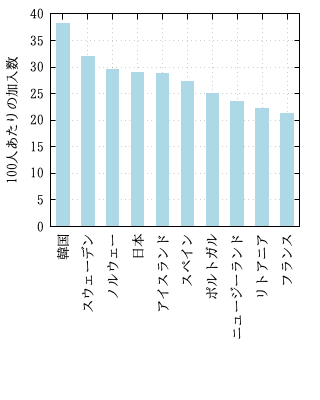
\includegraphics{fig11.png}
    \caption{光ファイバー回線の加入者(100人あたり)}\label{1}
\end{figure}
% 図の挿入
% \includegraphics{}
% を
% \begin{figure}[htbp]
% \end{figure}
% で囲み
% \caption{}
% で図のタイトルを入れる.
% \label{}
% を使って図番号が参照できるようにする
% また,
% \centering
% で図が中央に来るようにする

% ーーー
\section{デジタル競争ランキング}
% 節見出し(2)

国際経営開発研究所(IMD)の調査\cite{imd}によると、表\ref{2}に示すように、
日本のデジタル競争力のランキングは調査対象の64カ国中、総合で
28位、知識分野で25位となっている。
% 本文(2)
\begin{table}[htbp]
    \centering
    \caption{デジタル競争ランキング(64カ国中)}
    \label{2}

    \begin{tabular}{c|c|c}
        国 & 総合 & 知識 \\
        \hline
        米国 & 1位 & 3位 \\
        \hline
        香港 & 2位 & 5位 \\
        \hline
        スウェーデン & 3位 & 2位 \\
        \hline
        デンマーク & 4位 & 8位 \\
        \hline
        シンガポール & 5位 & 4位 \\
        \hline
        韓国 & 12位 & 15位 \\
        \hline
        中国 & 15位 & 6位 \\
        \hline
        日本 & 28位 & 25位 \\
        \hline
    \end{tabular}
\end{table}

% 表の挿入
% \begin{tabular}
% \end{tabular}    
% による表の記述を 
% \begin{table}[htbp]
% \end{table}
% で囲み
% \caption{}
% で表のタイトルを入れる.
% \label{}
% を使って表番号が参照できるようにする
% また,
% \centering
% で表が中央に来るようにする

% ーーー
\section{考察}

% 見出し(3)
% 考察
\begin{itemize}
    \item ブロードバンドの整備状況が良くてもデジタル競争力ランキングはあまり高くない国もある
    \item デジタル競争力ランキングの総合と知識部門では多少ズレはあるものの上位国は大体同じである
\end{itemize}
% \begin{itemize}
% \end{itemize}
% を使って箇条書きで記述する

% ここに参考文献が入る
%
\bibliographystyle{junsrt}
\bibliography{exercise.bib}

\end{document}